\chapter{Advanced orientation}



%=======================================================================================================
\section{Creating a calibration unknown by image}

  % - - - - - - - - - - - - - - - - - - - - -
\subsection{When is it necessary?}

It sometimes happens that each image, or each group of images,
has been acquired with a different set of internal parameters. Here
are possible cases:

\begin{itemize}
    \item when images were acquired with autofocus, which creates variation
          of the focal length (in macro photo, the focal length when focus is
          at $\infty$ is half the focal length when the focus is at image ratio of $1:1$),


    \item when  the image stabilizer is free, this creates (at least)
          variation of principal point;

    \item when  images were acquired with variable zoom.
\end{itemize}


From a photogrammetric point of view, these cases must be avoided
as much as possible; however there are times when the user has no
choice.

  % - - - - - - - - - - - - - - - - - - - - -
\subsection{Examples}

The directory {\tt applis/XML-Pattron/Oiseau-Margot/} contains XML
files that were used to process images acquired with macro lenses.
The files {\tt New-Apero1.xml} to {\tt New-Apero6-ExportDirPlanMM.xml}
contain examples on real cases of the different mechanisms shown
here. By the way, these examples may be a bit complex because they
were made before key standardization.

See especially the examples {\tt Apero-ExCalibPerIm-1.xml} and
{\tt Apero-ExCalibPerIm-2.xml} on {\tt MurSaintMartin}, that have
been added after writing this section; they are more realistic
and contain some comments at the beginning that should be
sufficient.

  % - - - - - - - - - - - - - - - - - - - - -
\subsection{How to create unknowns}

The optional section {\tt <CalibPerPose>}, under {\tt <CalibrationCameraInc>},
allows to handle these cases. It contains a mandatory args {\tt   <KeyPose2Cal>}:


\begin{itemize}
    \item it must contain a string $K$ which describes  a key association,
          (see~\ref{Ref:Key:Map}  for {\tt <KeyedNamesAssociations>});
    \item  two images  $I_1$ and $I_2$ will share the same internal parameters,
           if and only if $K(I_1) = K(I_2)$;
     \item for example,  if $K$ is the identity key, a new calibration will
           be created for each new image;

     \item  for each of these calibrations, the identifier will be $K(I)$ and not,
            as usual, the tag {\tt <Name>}; this is necessary because elsewhere
             different internal calibration would have the same identifier;

      \item this identifier is used when it is necessary to refer
            to a set of internal calibration (for example when applying
            constraint only to a subset of the existing calibration);

\end{itemize}

  % - - - - - - - - - - - - - - - - - - - - -
\subsection{Saving  results with  variable calibrations}

The most current case for using these mechanisms is when there is one calibration
per image. In this case, the easiest way for handling the results is  to
simply  save the internal calibration  with the external calibration;
this is, by default, what Apero does  in {\tt <ExportPose>}, see
{\tt Apero-0.xml} in~\ref{Result:Apero0}.


For more complicated cases,  an {\tt <ExportCalib>} section  will have to be
used with the following tags:

\begin{itemize}
    \item {\tt <PatternSel>}  to specify to which calib it applies; the selection
         is made on the identifier (here $K(I)$);

    \item {\tt <KeyAssoc>}  to specify how to compute a file name from the identifier;

    \item {\tt <KeyIsName>}  at {\tt false} \footnote{which is, however, the default value} meaning
          that {\tt <KeyAssoc>}  is a key and not an absolute name;
\end{itemize}


  % - - - - - - - - - - - - - - - - - - - - -
\subsection{Loading initial values  with  variable calibrations}

When  variable internal calibration is used a first time,
the different calibration can be initialized with the same
value.  This value can be read as usual in the {\tt <NameFile> } of {\tt <CalValueInit>}.
See an example in {\tt  applis/XML-Pattron/Oiseau-Margot/New-Apero1.xml},

There is other cases where it will be needed to initialize these  calibrations
from variable values; for example, values  that have been computed and saved by a
previous running of Apero. In this case, a {\tt KeyedNamesAssociations} will be used
to specify the association between \emph{the  name of the pose} and the file where
the initial value is to be read; this key is specified in the optional
{\tt <KeyInitFromPose>}; see example in {\tt  applis/XML-Pattron/Oiseau-Margot/New-Apero3.xml}.


\subsection{Examples with group of poses}

Sometimes we do not want to create a calibration for each image,
but a calibration for each group of images. This can occur
when we know that the parameters affecting the calibration
(zoom, focus) have changed, but only a few times, and we are able
to specify which groups of images share the same parameters.
This can also occur when we have used several versions of the
same camera with the same focal length (so not distinguishable
with the procedure used in {\tt Tapas}).

See {\tt Apero-ExCalibPerGROUPIM-1.xml} and
{\tt Apero-ExCalibPerGROUPIM-2.xml}  on  {\tt MurSaintMartin} data
set, it illustrates how this can be done. The file contains
some comments.


The files {\tt Apero-ExCalibPerIm-1.xml} and {\tt Apero-ExCalibPerIm-2.xml}
on  {\tt MurSaintMartin} have been added and contain also
examples for calibration per images which are probably easier to understand
than {\tt  applis/XML-Pattron/Oiseau-Margot/}.

%=======================================================================================================

\section{Database of existing calibration}

\label{DB:Calib}
\subsection{General points}


%=======================================================================================================
\section{Auxiliary exports}

  % - - - - - - - - - - - - - - - - - - - - -

\subsection{Generating point clouds with {\tt <ExportNuage>}}

\label{Ap:Exp:Nuage}


%=======================================================================================================

\section{Using scanned analog images}

\label{Analog:Image}
Scanned analog images are important in many applications, as they represent
a valuable source of information for studying phenomena on long periods of time.
From the photogrammetric point of view, the main difference between
scanned images and digital camera is that for each images there
is a specific  transformation between the photo and the scanner.
This transformation can be computed when there exist fiducial marks
on the camera. This section presents how this can be done with {\tt Apero/MicMac}.


The directory {\tt DemoScanned/} contains a data set that illustrates these
features. It contains $5$ images that are a simulation of scanned
images: the images have been randomly rotated and scaled, simulating the
interior orientation of the scanner; before the rotation, $8$  fiducial marks have
been added. Figure~\ref{ImFid} illustrates this data set.


\begin{figure}
\begin{tabular}{||c|c||}
   \hline \hline
   \multicolumn{2}{c|}{\includegraphics[width=120mm]{FIGS/Niche/ImGlob.jpg}} \\
   \includegraphics[width=40mm]{FIGS/Niche/Cible1.jpg} &
   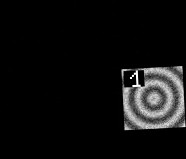
\includegraphics[width=40mm]{FIGS/Niche/Cible2.jpg}
\end{tabular}
\caption{Simulation of fiducial marks: an image and two marks }
\label{ImFid}
\end{figure}


There are two slight differences in data processing between such data sets and "classical" digital images:


\begin{itemize}
   \item the position of fiducial mark on images and on the camera has to be indicated;
   \item the calibration will not be expressed in pixel, but in the same unit
         as the position of the reference fiducial marks (generally $mm$).
\end{itemize}

On {\tt DemoScanned/}, the directory {\tt Ori-InterneScan/} contains all the information
about the fiducial marks. It works like this:

\begin{itemize}
    \item each file contains a structure, a type {\tt <MesureAppuiFlottant1Im>} which describes a list
          of named points (here the names are {\tt P0, P1, \dots}; this is the same structure as the one used
          for image measurement of GCP, as seen in~\ref{GCP:Org};

     \item there is a file {\tt MeasuresCamera.xml} that contains the position of the fiducial marks
          on the camera;

     \item for each image {\tt XXX}, there is a file {\tt MeasuresIm-XXX.xml} that contains the position
           of the marks on the image; when this file does not exist, the image is considered to be a "classical"
           digital image that will be processed as usual;

     \item if required\footnote{for example if several analog camera are used in the same bundle},
           it is possible to change the association between an image and the two files: position in camera
           and image; for this, you must change the  value of {\tt Key-Assoc-STD-Orientation-Interne}
           \footnote{see in include/XML\_GEN/DefautChantierDescripteur.xml the default value}
           in your {\tt MicMac-LocalChantierDescripteur.xml}
\end{itemize}

Here, the file {\tt MeasuresCamera.xml} contains the positions of fiducial marks in $mm$,
all the calibration  must then be have the same unit and be in the same frame than these
marks. For technical reasons, this point of reference must be the upper left corner and not the center.
As {\tt Apero/MicMac} cannot deal correctly with default calibration in $mm$, we
have to give an initial value in file {\tt Ori-CalibInit}. Some comments on this file:

\begin{itemize}
    \item  the size of image {\tt <SzIm>} is also in $mm$ (as the normalization focal
            {\tt <Etats>}  and all parameters).
     \item  the optional {\tt  <ScannedAnalogik> } is set to true, required because
            it will indicate to {\tt Apero} to be "tolerant" if tie points are detected out
            of the bounding box $[0,0]x[24,36]$;
\end{itemize}

The file {\tt ExCmd.txt} contains a possible processing of the data:


\begin{itemize}
    \item {\tt Tapioca  All ".*jpg"  1200}, as usual \dots
    \item {\tt Tapas  FishEyeBasic  ".*jpg"  Out=Ori1 InCal=CalibInit PropDiag=0.68}

     \begin{itemize}
          \item  it is necessary to indicate the calibration in {\tt CalibInit} in $mm$ because {\tt Apero}
                 would not built it correctly;
          \item no need to indicate situation of fiducial mark, the def value of {\tt Key-Assoc-STD-Orientation-Interne}
                will force {\tt Apero} to look for them at the right place;
           \item {\tt PropDiag=0.68} , because it is a hemispheric fisheye;
      \end{itemize}

    \item {\tt Tapas FishEyeBasic ".*jpg" InOri=Ori1  Out=Ori2 PropDiag=0.68}
    \begin{itemize}
           \item  just to check that {\tt Tapas} can be iterated in  this  configuration
    \end{itemize}
    \item {\tt Malt GeomImage ".*jpg" Ori2 Master=IMG\_5693\_Out.jpg Spherik=true SzW=2}
    \begin{itemize}
             \item the {\tt Spherik=true} is well adapted  to the scene, in this geometry
                   {\tt MicMac} computes the depth  $R=f(i,j)$ where $R$ is the distance
                   to the master image center \footnote{i.e. rectification is made on sphere};
    \end{itemize}

    \item {\tt Nuage2Ply MM-Malt-Img-IMG\_5693\_Out/NuageImProf\_STD-MALT\_Etape\_8.xml Attr=IMG\_5693\_Out.jpg Scale=2}

    \begin{itemize}
             \item usual generation of point cloud in ply format (figure~\ref{ImNiche});
    \end{itemize}

\end{itemize}




\begin{figure}
   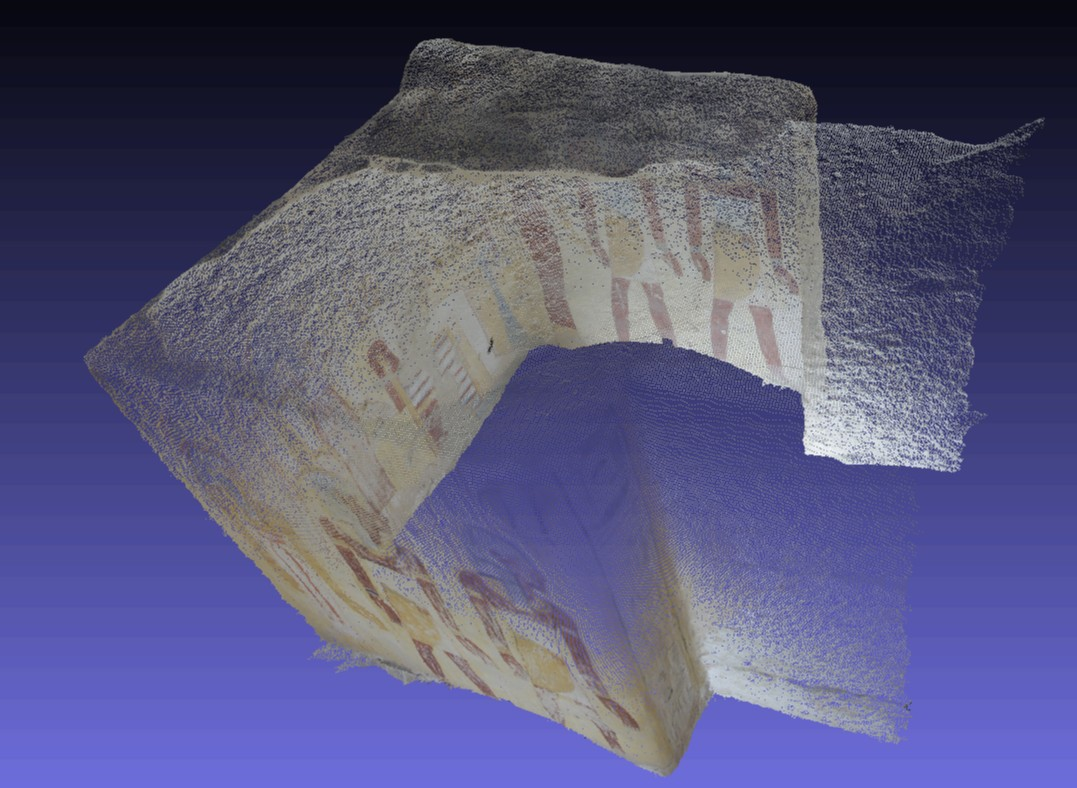
\includegraphics[width=120mm]{FIGS/Niche/snapshot00.jpg}
\caption{Point cloud with simulation of scanned images}
\label{ImNiche}
\end{figure}


If you take a look at orientation files, you will see that they are self sufficient for
matching: the {\tt <OrIntImaM2C>}  section contains the affinity between scanner and image computed
from the fiducial marks:

\begin{verbatim}
     <OrientationConique>
...
          <OrIntImaM2C>
               <I00>2753.06179948014324 1771.95961861625119</I00>
               <V10>-72.5948450058228758 4.58183503308403939</V10>
               <V01>-4.5818350330840607 -72.5948450058228332</V01>
          </OrIntImaM2C>
...
     </OrientationConique>
\end{verbatim}


%=======================================================================================================

\subsection{Semi-automatic fiducial mark input with Kugelhupf}

Kugelhupf (Klics Ubuesques Grandement Evites, Lent, Hasardeux mais Utilisable pour Points Fiduciaux) is a tool for scanned images. It is used to automatically find fiducial marks on the images.

If the fiducial marks are almost on the same position on each picture, it is necessary to point them on one image and Kugelhopf will find the fiducial marks on the others.

Syntax of {\tt Kugelhupf}:
\begin{verbatim}
*****************************
*  Help for Elise Arg main  *
*****************************
Mandatory unnamed args : 
  * string :: {Pattern of scanned images}
  * string :: {2d fiducial points of an image}
Named args : 
  * [Name=TargetHalfSize] INT :: {Target half size in pixels (Def=64)}
  * [Name=SearchIncertitude] INT :: {Search incertitude in pixels (Def=5)}
  * [Name=SearchStep] REAL :: {Search step in pixels (Def=0.5)}
\end{verbatim}

Call example:
{\tt mm3d Kugelhupf "1987\_FR4074.*.tif" Ori-InterneScan/MeasuresIm-202.tif.xml SearchIncertitude=10 }

The output is xml files in {\tt Ori-InterneScan} for every picture where the automatic search was successful.
If at least one point was not found for an image, the xml file is not created.
Kugelhupf only works on picture that have no xml file.

This is useful to make successive calls to Kugelhupf with different search incertitudes :

{\tt mm3d Kugelhupf "1987\_.*.tif" Ori-InterneScan/MeasuresIm-202.tif.xml SearchIncertitude=10}

{\tt mm3d Kugelhupf "1987\_.*.tif" Ori-InterneScan/MeasuresIm-202.tif.xml SearchIncertitude=25}


The first call will be fast and will have a result only with pictures with close fiducial points, and the second call will
be slower but only on the worst pictures.


\section{Adjustment with lines}


        % - - - - - - - - - - - - - - - - - - - - - - - - - - - - - - - - - - - - - - -

\subsection{Introduction}

This section describes the case where user wants to adjust orientation using correspondence between $3d$ points
and image lines. It's rather specific, and was added in the context of georeferencing aerial photographs with a $3d$
data base of roads \footnote{I am not sure to see if there exist other examples of application}. Formally we have:

\begin{itemize}
    \item a set of $2d$ line $L_k$ in images. Let $I_k$ be the corresponding image and $\pi_k$ be the projection
         function that goes from ground coordinates to $I_k$;
    \item for each $3d$ point a set of point $p_{k,i}$ and we "know" that $\forall k,i \, : \pi_k (p_{k,i}) \in L_k $
    \item let $D(p,L)$ be the distance between point $p$ and line $L$.
\end{itemize}

Mathematically we want to add the cost to the global minimization:

\begin{equation}
    \sum_{k,i} D^2 ( \pi_k(p_{k,i}),L_k) \label{EQU:LINE:POINT}
\end{equation}


        % - - - - - - - - - - - - - - - - - - - - - - - - - - - - - - - - - - - - - - -

\subsection{Data set}

The folder {\tt Documentation/NEW-DATA/CompensOnLine/} contains  data that illustrates how this can be done in
{\tt Apero}. These are completely artificial (simulated) data which were generated for developing and testing this feature: in this example it will be possible to cancel completely the equation~\ref{EQU:LINE:POINT} which will obviously not
be the case with real data.

To run the data set extracted from the mercurial server, one first needs to compute the tie points with:

\begin{itemize}
   \item {\tt mm3d Tapioca All Abbey-IMG\_020.*jpg 1200}
\end{itemize}

To test all features, this data set has been processed as if it was the scans of analog images
(see {\tt Ori-InterneScan/}), but it also works with digital images. As it can be seen in {\tt mm3d-LogFile.txt},
the orientation has been computed with the command:

\begin{itemize}
   \item {\tt mm3d Tapas AutoCal Abbey-IMG\_020.*jpg InCal=Ori-CalibInitAnalogik/ Out=Rel}

\end{itemize}

This toy example is made from $4$ small images on the same strip. Of course the data are completely  artificial:

\begin{itemize}
   \item when using the "real" orientation (i.e Ori-Rel/) the projection of point on lines is perfect;
   \item there exist data for each image;
   \item for each images the data is sufficient to compute its orientation;
\end{itemize}

        % - - - - - - - - - - - - - - - - - - - - - - - - - - - - - - - - - - - - - - -

\subsection{Organization of information}

Basically, the information is structured the same way as for GCP in~\ref{GCP:Org},\ref{Sec:GCPBascule} and
\ref{CAMPARI} :

\begin{itemize}
   \item there is a file for storing the $3d$ point, in this example {\tt MesurePointGround.xml}, it is the same
         structure that for {\tt GCP}, and the adjustment of this point can mix measurement of $3d$ in ground,
         $2d$ points in images and $2d$ lines in images;

   \item there is a file for storing $2d$ images line coordinates and the points that are supposed to project
         on these lines, in this example {\tt MesureLineImage.xml};

   \item in {\tt Apero} these files are loaded, linked and then used for adjustment.
\end{itemize}

The structure of {\tt MesureLineImage.xml} should be quite obvious:

\begin{itemize}
   \item it must contain a global structure {\tt <SetOfMesureSegDr>};
   \item the {\tt <SetOfMesureSegDr>} is a list of {\tt <MesureAppuiSegDr1Im>}, each one
         storing the observation related to one image;
   \item a  {\tt MesureAppuiSegDr1Im} contains the name of the image {\tt <NameIm>}, and list a of {\tt <OneMesureSegDr>}, each one storing the information related to a line;

   \item a   {\tt <OneMesureSegDr>} contains exactly two $2$ points {\tt <Pt1Im>} and {\tt <Pt2Im>} that store
            the geometry of the line and a list of {\tt <NamePt>} that contains the name of the $3d$ points;
            there can be any number $N \geq 1$ of  {\tt <NamePt>} , even if in this example we
             have $N=2$ everywhere
             \footnote{which will probably be the standard case when the $3d$ points come from $3d$ lines}.

\end{itemize}

        % - - - - - - - - - - - - - - - - - - - - - - - - - - - - - - - - - - - - - - -

\subsection{Example {\tt Apero-2-DroiteStatique.xml}}

\label{Apero-2-DroiteStatique}

It illustrates file loading.
In this example, we only load the observation and check that the projection is perfect (because data
are simulated). It's pretty much the same than~\ref{GCP:Org} :

\begin{itemize}
   \item {\tt BDD\_ObsAppuisFlottant} load the line information, in a data base name {\tt Id-Appui};
         the name of the file containing the line is stored in {\tt  <KeySetSegDroite>};
   \item {\tt PointFlottantInc} load the $3d$ points information, in the same data base {\tt Id-Appui};
   \item {\tt ObsAppuisFlottant} add the observation of the data base {\tt Id-Appui} to the adjustment.
\end{itemize}

As in this example the data are all frozen \footnote{see {\tt ePoseFigee} and {\tt eAllParamFiges}}, we just print the
value of the observed distance, which turns to b $0$ up to the rounding error. We obtain the error for each point, and
the maximum of error :


\begin{verbatim}
...
    ErrMax = 1.65784e-11 For I=Abbey-IMG_0205.jpg,  C=P_8_B pixels
  - - - - - - - - - - -
==== ADD Pts P_9_A Has Gr 1 Inc [1,1,1]
--NamePt P_9_A Ec Estim-Ter [0,0,0]           Dist =0 ground units
Inc = [1,1,1]PdsIm = [1,1]
    Ecart Estim-Faisceaux 16.2788
      ErrMoy 2.71776e-13 pixels  SP=2
     ErrMax = 2.71776e-13 For I=Abbey-IMG_0204.jpg,  C=P_9_A pixels
  - - - - - - - - - - -
==== ADD Pts P_9_B Has Gr 1 Inc [1,1,1]
--NamePt P_9_B Ec Estim-Ter [0,0,0]           Dist =0 ground units
Inc = [1,1,1]PdsIm = [1,1]
    Ecart Estim-Faisceaux 16.1819
      ErrMoy 6.65003e-12 pixels  SP=2
     ErrMax = 8.11932e-12 For I=Abbey-IMG_0205.jpg,  C=P_9_B pixels
  - - - - - - - - - - -

   ============================= ERRROR MAX PTS FL ======================
   ||    Value=4.56508e-10 for Cam=Abbey-IMG_0204.jpg and Pt=P_2_A
   ======================================================================
\end{verbatim}

        % - - - - - - - - - - - - - - - - - - - - - - - - - - - - - - - - - - - - - - -

\subsection{Example {\tt Apero-3-DroiteEvolv.xml}}

In this example, we  want to check that with "perfect" data, the adjustment on line
is sufficient to compute the "perfect" orientation as long as we are reasonably initialized.
It's pretty much the same than~\ref{Apero-2-DroiteStatique},
except that we start from start from orientation that have been modified and
do not freeze the orientation.


\begin{verbatim}
...
  ============================= ERRROR MAX PTS FL ======================
   ||    Value=16.9249 for Cam=Abbey-IMG_0207.jpg and Pt=P_13_A
   ======================================================================
--- End Iter 0 ETAPE 0
...
...
   ============================= ERRROR MAX PTS FL ======================
   ||    Value=0.00335622 for Cam=Abbey-IMG_0207.jpg and Pt=P_13_A
   ======================================================================
--- End Iter 1 ETAPE 0
...
...
   ============================= ERRROR MAX PTS FL ======================
   ||    Value=8.87999e-09 for Cam=Abbey-IMG_0204.jpg and Pt=P_14_B
   ======================================================================
--- End Iter 2 ETAPE 0
...
...
   ============================= ERRROR MAX PTS FL ======================
   ||    Value=3.17978e-10 for Cam=Abbey-IMG_0204.jpg and Pt=P_2_A
   ======================================================================
--- End Iter 3 ETAPE 0
...
...
   ============================= ERRROR MAX PTS FL ======================
   ||    Value=3.17775e-10 for Cam=Abbey-IMG_0204.jpg and Pt=P_2_A
   ======================================================================
--- End Iter 4 ETAPE 0

\end{verbatim}

At the end, the orientation are exported in {\tt Ori-Check3/}, and it can be seen that they are almost identical to {\tt Ori-Rel}


        % - - - - - - - - - - - - - - - - - - - - - - - - - - - - - - - - - - - - - - -

\subsection{Example {\tt Apero-4-CompensMixte.xml} and  {\tt  Apero-5-CompensAll.xml}}

In this example, we check that, as we would do in real case, it is possible to adjust simultaneously GCP-line with
other measurement. Also we use a reduced set of line-point (with {\tt MesureLineImageIncompl.xml}), in this set
there is lines only for the two central images.

In {\tt Apero-4-CompensMixte.xml} we check that using simultaneously tie point and "GCP-line", we can recover the orientation
of the extreme images (where there is no GCP-line).

{\tt  Apero-5-CompensAll.xml} had a minor modification, we see that in {\tt <BDD\_ObsAppuisFlottant >} we have

\begin{itemize}
   \item  {\tt <KeySetSegDroite> } as before , to make adjustment on line;
   \item an additional {\tt  <KeySetOrPat>} to make adjustment of $2d$ points like in  ~\ref{GCP:Org};

\end{itemize}

So in this example, the $3d$ point {\tt P\_1\_A} will be adjusted simultaneously on:

\begin{itemize}
    \item $2d$ point measure stored in {\tt MesurePointImagePart.xml};
    \item $2d$ line measure stored in {\tt MesureLineImage.xml};
    \item $3d$ point measure stored in {\tt MesurePointGround.xml}.
\end{itemize}

%=======================================================================================================
\section{Recent evolution in Tapas and other orientation tools}

The evolution described here, are now integrated in the "standard" {\tt Tapas} command.
When necessary \footnote{for example because "new"  {\tt Tapas} has slower convergence}, it is possible
to get back to the previous behavior by using the {\tt OldTapas} command.



        % - - - - - - - - - - - - - - - - - - - - - - - - - - - - - - - - - - - - - - -

\subsection{Viscosity \& Levenberg Marquardt stuff}

Adding viscosity, also named more pedantically using Levenberg Marquardt algorithm,
is a classical way to avoid problem due to ill conditioning system in energy minimization algorithm.
In theory the only drawback is that it slow down the speed of convergence.

However, in Tapas, the default value of viscosity was badly dosed, and it  some configuration ,
particularly UAV acquisition \footnote{because it's big data set and the "loop is not closed}
lead to stop the bundle adjustment before the convergence . This is illustrated in figure~\ref{ImOldNewTapas}.
 To change this fact, the comportment of Tapas/NewTapas has evolved this way :

\begin{itemize}
    \item  the initial default value of viscosity  on center and rotation has been divided by $10$;
    \item  conversely the constraint to solve the arbitrary ambiguity has bee reactivated (i.e the first image is
           frozen, and the length of the base between two first images is frozen)
    \item  a small initial viscosity has been added on internal parameters;
    \item  in the third {\tt <EtapeCompensation>} the viscosity is continuously decreasing;
    \item  in the fourth step of  {\tt <EtapeCompensation>} the viscosity is highly strongly decreasing and
           the bundle does not stop before a test of convergence is satisfied (the test verify that with an
           accuracy of $1E-10$ the $3d$ point are identical after two consecutive steps).
\end{itemize}

As this new version can increase significantly the computation, the option {\tt RefineAll=false}
allow to limit the number of iteration (by a factor around $2$), of course it has a risk of non convergence \dots


\begin{figure}
\begin{center}
   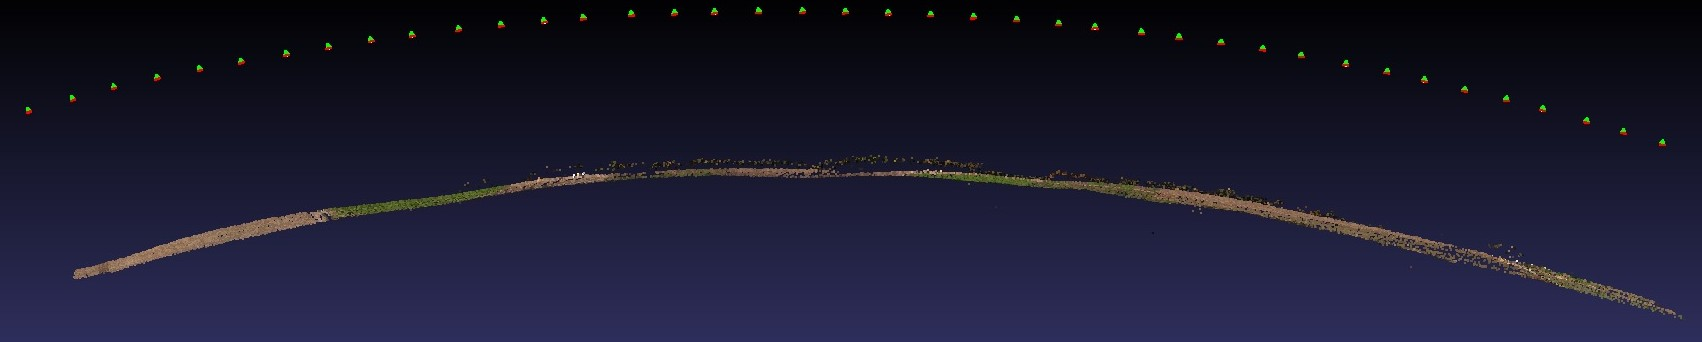
\includegraphics[width=120mm]{FIGS/NewTapas/Old00.jpg}
   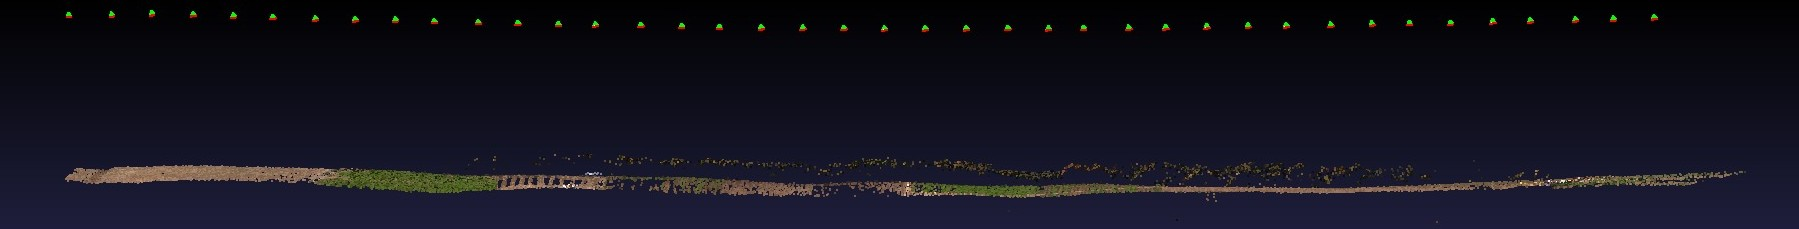
\includegraphics[width=120mm]{FIGS/NewTapas/New00.jpg}
\end{center}
\caption{Result with old and new version of Tapas, with first convergence is visibly not achieved}
\label{ImOldNewTapas}
\end{figure}


        % - - - - - - - - - - - - - - - - - - - - - - - - - - - - - - - - - - - - - - -

\subsection{Additional distortion}

The kernel of Apero has two option that can be useful when attempting to modelize finely camera distortion:

\begin{itemize}
   \item model with high degree of freedom
   \item possibility to define a distortion as composition of several distortion (as described in~\ref{ComposDist}).
\end{itemize}

These option are now partly accessible in Tapas.

There is two family of distortion with high degree of freedom :


\begin{itemize}
   \item high radial distortion made from a polynomial radial distortion and $6$ parameters for degree $2$
         general polynoms; these polynoms are available in Tapas via the {\tt Four7x2, Four11x2, Four15x2, Four19x2}
         and in Apero with {\tt eModeleRadFour7x2, ..., eModeleRadFour19x2}, the {\tt Four19x2} modelize the radial
         distortion with a polynom $r_3 \rho^3 +\dots + r_{19} \rho^{19}$; also I am not sure it maybe necessary to
         use until $ \rho^{19}$, I observe that with modern camera using sophisticated aspherical lenses, it may be
         insufficient to use the so called $r_3 r_5 r_7$ model;


   \item general polynomial model, i.e $D_N(X,Y) \sum (A_{i,j} x^iy^j,B_{i,j} x^iy^j)$  where $i+j\leq N$,
         there accessible in {\tt Apero} a a unified model {\tt eModelePolyDeg2, \dots eModelePolyDeg7},
         for example,{\tt eModelePolyDeg7} has $66$ parameters, because $66=8*9-6$, the $-6$ comes because
         there $6$ polynoms already modelized by focal, principal point and rotations;
\end{itemize}

The first one is accessible directly in {\tt Tapas}, not the second. But both are accessible as additional distortion.
In fact, it would be generally a bad idea to try to estimate directly the $66$ parameters of a {\tt eModelePolyDeg7}, it's
preferable to estimate first a model with physical meaning and few parameters, and then to estimate the high degree polynom as a modification to this physical model. This can be done with :

\begin{itemize}
    \item  {\tt AddFour7x2,  \dots AddFour15x2} for high degree radial models;
    \item  {\tt AddPolyDeg2, \dots AddPolyDeg7} for high degree general models;
\end{itemize}

A possible example of use :

\begin{verbatim}
"mm3d" "NewTapas" "Four15x2" "R.*JPG" "DegGen=2"
"mm3d" "NewTapas" "AddPolyDeg7" "R.*JPG" "InOri=Ori-Four15x2/"
\end{verbatim}

The first call is classical, just remark the {\tt DegGen=2} because by default only $1$ degree
general parameter od {\tt Four15x2} is free.  In the second call we start from the first orientation/calibration
and add a $7$ degree general polynom. Note that, as with {\tt AutoCal} et {\tt Figee} all the calibration must have
an initial value when using the additional mode.

Also note that only the additional distortion will be optimized (else the problem would be far over parameterized).
The result in {\tt Ori-AddPolyDeg7/AutoCal60.xml} looks like :

{\tiny
\begin{verbatim}
<ExportAPERO>
     <CalibrationInternConique>
          <KnownConv>eConvApero_DistM2C</KnownConv>
          <PP>389.315403456829813 291.190537211471565</PP>
          <F>653.34645310282724</F>
          <SzIm>800 600</SzIm>
          <CalibDistortion>
               <ModUnif>
                    <TypeModele>eModeleRadFour15x2</TypeModele>
                    <Params>0.000731887299586956555</Params>
      .....
                    <Etats>499.999999999999943</Etats>
                    <Etats>399.999999999999943</Etats>
                    <Etats>300</Etats>
               </ModUnif>
          </CalibDistortion>
          <CalibDistortion>
               <ModUnif>
                    <TypeModele>eModelePolyDeg7</TypeModele>
                    <Params>-0.00116060037632004101</Params>
                    <Params>0.000376819315728853894</Params>
      .....
                    <Params>0.155804133319492222</Params>
                    <Etats>652.861598677042821</Etats>
                    <Etats>391.129060939043825</Etats>
                    <Etats>287.689359319814059</Etats>
               </ModUnif>
          </CalibDistortion>
     </CalibrationInternConique>
</ExportAPERO>

\end{verbatim}
}

        % - - - - - - - - - - - - - - - - - - - - - - - - - - - - - - - - - - - - - - -

\subsection{Non Linear Bascule (swing)}

\subsubsection{Motivation}

\label{NonLin:GCPBascule}

The {\tt GCPBascule} tool, described in~\ref{Sec:GCPBascule}, transforms a relative orientation
into an absolute one, using at least $3$ ground control point (GCP). The default use make
the assumption that the relative orientation is "perfect" and it computes the minimum number
of parameters, i.e. the seven parameter corresponding to the arbitrary $3d$ similitude
 that can be computed from tie points :

\begin{itemize}
   \item $3$ parameter for rotation;
   \item $3$ parameter for translation;
   \item $1$ parameter for scale.
\end{itemize}


When {\tt MicMac} tools is used for metrology, this geo-referencing by {\tt GCPBascule}
can be insufficient because there appears non linear distortion in the relative orientation. The discussion about the
origin and the quantification of these effect,  is quite complex and cannot be discussed here;
however,  to solve it we have to input more GCP that the minimum required and to use these
surplus GCP for correcting this distortion. In {\tt MicMac} tools, there is two way to do it :


\begin{itemize}
   \item the "classical" way is to do a compensation with high weighting on the GCP, this can be done
        with the simplified tool   {\tt Campari}  (\ref{CAMPARI} and \ref{Bundle:CAMPARI});

   \item a non standard way is to use the redundancy of the GCP to directly estimate the non linear distortion
        existing between the result of "Bascule" (swing) ans the ground truth; this is what is described here;

\end{itemize}

At the time of writing these documentation, it's not clear which method is "better". The first one is more
standard and seems more correct from theoretical point of view, however from experimental point of view, the
second one seems more accurate.


\subsubsection{Mathematical model}

Let :

\begin{itemize}
   \item let $G_k$ be the ground coordinate of the GCP;
   \item let $I_k$ be the coordinate of the GCP in relative initial model (estimate by bundle intersection);
   \item let $T$ be the transformation from relative to absolute we want to estimate similitude, such that  $G_k \approx T(I_k)$ ;
   \item let $S$ be the initial similitude estimation of $T$;
   \item let $C$ be the "small" correction we want to do compute $T= (Id+C) \circ S$
\end{itemize}


Also, it is current that the acquisition is "linear" and that the coordinate must not be treated
symmetrically. For example if the acquisition is made from a single strip, let $O'X'Y'Z$ be a
coordinate system ,  centered on the acquisition, such that the image center are aligned on the $O'X'$ axes.
Concretely $O'X'Y'Z$ can be estimated automatically from initial $OXYZ$ by elementary computation of inertial axes of the
image center (i.e. computation of order $2$ moments) \footnote{this is exactly what is done in MicMac}.



Basically, the model for estimate $C$ is restricted  quadratic function on of  each coordinates $X'Y'Z$:

\begin{itemize}
   \item $C(X',Y',Z') = (X'^c,Y'^c,Z'^c)$;
   \item $X'^c = \sum c^x_{ij} X'^i Y'^j$
   \item $Y'^c = \sum c^y_{ij} X'^i Y'^j$
   \item $Z'^c = \sum c^z_{ij} X'^i Y'^j$
\end{itemize}


For example, suppose that the acquisition is made from a single strip, and
that the errors is only on $Z^c$,  and that this error depends only on  the
"main" variable $X'$, a possible mode could be :

\begin{itemize}
   \item $X'^c = 0$
   \item $Y'^c = 0$
   \item $Z'^c =  c^z_{00} + c^z_{10} X' + c^z_{20} X'^2$
\end{itemize}

Also if we have a sufficient number of tie points \footnote{$6$ is the minimum, but $12$ would be more
reasonable} and have high distortion we can select the full model.


\subsubsection{Using it in MicMac}

The command {\tt GCPBascule} has several parameters to compute a non linear
correction. Of course by default, the swing-bascule if made with the standard $7$ parameters
with no correction. The non linear correction is activated if the optional {\tt PatNLD} is
used. The meaning of the different parameters is then :


\begin{itemize}
  \item  {\tt PatNLD} :  define the pattern of the GGP name that will be used to estimate  $C(X',Y',Z')$;
         in the final application probably one will use {\tt "PatNLD=.*"} to specify that all GCP; however,
         if one want to estimate the accuracy with GCP that are not used for the estimation, it can be
         convenient to specify a subset:
   \item  {\tt NLDegX}, {\tt NLDegY} and  {\tt NLDegZ} specify the monoms that be used for  $X'^c,Y'^c,Z'^c$,
          it a vector of strings  which elements must belongs to {\tt \{1,X,Y,X2,XY,Y2\}};
   \item  {\tt NLFR}  : as the function $T$ is no longer a pure similitude, the orientation of each image
          can no longer be exactly a rotation matrix; the parameter {\tt NLFR} mean "Non Linear For Rotation" and
          control the export is done ; if :

\begin{itemize}
     \item   {\tt NLFR} is false, {\tt MicMac} will export for each image the closest matrix that fit
             with new system, if $X'^c,Y'^c,Z'^c$ contains non linear term there will be some error but
             probably very small; the matrix will be non rotation matrix which mean that there will be
             no longer usable compensation (but usable in matching);

     \item   {\tt NLFR} is true, {\tt MicMac} will export for each image the closest rotation that fit
             the new system; of course the price to pay for having true rotation is that the error will be bigger;

\end{itemize}

   \item  {\tt NLShow}  : give detailed information;
\end{itemize}




\subsubsection{Example of use, and message interpretation}

Here is a possible use :

{\small
\begin{verbatim}
 "mm3d" "GCPBascule" ".*ARW" "Ori-AllRell-F15AddP7/" "Basc-Def-NonO" "GCP.xml" "MesFinal-S2D.xml" \
   "PatNLD=(3|7|14).*" "NLDegZ=[1,X,X2]" "NLDegX=[1,X,Y]" "NLDegY=[1,X,Y]" "NLFR=false" "NLShow=true"
\end{verbatim}
}

The message should look like that , first classical message of {\tt GCPBascule} :

\begin{verbatim}
BEGIN Pre-compile
NEW CALIB TheKeyCalib_350
NB[10a]= 11
  .....
NB[9c]= 11
BEGIN Load Observation
Pack Obs NKS-Set-Orient@-AllRell-F15AddP7 NB 180
BEGIN Init Inconnues
NUM 0 FOR 001aDSC01061.ARW
  .....
NUM 179 FOR 242bDSC01005.ARW
BEGIN Compensation
BEGIN AMD
END AMD
\end{verbatim}

Then  a message remembering the monom used for $X'^c,Y'^c,Z'^c$ :

\begin{verbatim}
 MQ:X [1 X Y ]
 MQ:Y [1 X Y ]
 MQ:Z [1 X X2 ]
\end{verbatim}

Then the error before and after non linear correction :

\begin{verbatim}
* 14a ErInit : 0.0723239 => ErCor : 0.0260313 DZ=-0.0254591
* 14b ErInit : 0.043778 => ErCor : 0.0135564 DZ=0.00440725
* 14c ErInit : 0.0277668 => ErCor : 0.0253775 DZ=0.0211511
  13a ErInit : 0.0583578 => ErCor : 0.0456215 DZ=-0.042776
  13b ErInit : 0.0361378 => ErCor : 0.0231452 DZ=-0.0176777
  13c ErInit : 0.0200873 => ErCor : 0.020112 DZ=0.00742163
   ....
\end{verbatim}

Let detail the message for point {\tt  14a} :
\begin{itemize}

 \item {\tt * 14a ErInit : 0.0723239 => ErCor : 0.0260313 DZ=-0.0254591};
 \item the {\tt *} means that point {\tt  14a} belongs to {\tt PatNLD}
 \item {\tt 0.0723239} is the initial distance $||G_k - S(I_k)||$ (after bascule-swing);
 \item {\tt 0.0260313} is the distance after non linear correction $||G_k - T(I_k)||$ ;
 \item {\tt -0.0254591} is the $Z$ value of $||G_k - T(I_k)||$ (generally the most important);

\end{itemize}


        % - - - - - - - - - - - - - - - - - - - - - - - - - - - - - - - - - - - - - - -




        % - - - - - - - - - - - - - - - - - - - - - - - - - - - - - - - - - - - - - - -

\subsection{A detailed example}



%=======================================================================================================

\section{Miscellaneous  tools about calibration}

  % - - - - - - - - - - - - - - - - - - - - -

\subsection{{\tt ConvertCalib} to Calibration conversion}

Sometimes it may be necessary to export a given calibration from one model to another model. For example from Fraser terrestrial
model to aerial model. Of course as the mathematicall modelisation of the camera is not the same, this conversion will 
generally imlply some lost of accuracy.  The tool {\tt ConvertCalib} allow to do such conversion.

\begin{verbatim}
mm3d ConvertCalib
*****************************
*  Help for Elise Arg main  *
*****************************
Mandatory unnamed args : 
  * string :: {Input Calibration}
  * string :: {Output calibration}
Named args : 
  * [Name=NbXY] INT :: {Number of point of the Grid}
  * [Name=NbProf] INT :: {Number of depth}
  * [Name=DRMax] INT :: {Max degree of radial dist (def=depend Output calibration)}
  * [Name=DegGen] INT :: {Max degree of generik polynom (def=depend Output calibration)}
  * [Name=PPFree] bool :: {Principal point free (Def=true)}
  * [Name=CDFree] bool :: {Distorsion center free (def=true)}
  * [Name=FocFree] bool :: {Focal free (def=true)}
  * [Name=DecFree] bool :: {Decentrik free (def=true when appliable)}
\end{verbatim}


The first argument is a file containg the calibration to be converted. The second is a file that contain a model of the
targeted calibration. The folder {\tt Documentation/NEW-DATA/DocConvertCalib} contains data to test this tool :

\begin{itemize}
   \item  {\tt Aerial.xml} a calibration with aerial model ({\tt PPA} and {\tt PPS} separated);
   \item  {\tt Fraser-Affine.xml} a calibration with fraser model ({\tt PPA} and {\tt PPS} merged, decentric distorsion);
\end{itemize}

For example , if we want to produce a convertion to fraser model, without affine distorsion and a one parameter of radial
distorsion, we can run :

\begin{verbatim}
mm3d ConvertCalib Aerial.xml Fraser-Affine.xml  DRMax=1 DegGen=0
....
   ============================= ERRROR MAX PTS FL ======================
   ||    Value=0.145258 for Cam=Fraser-Affine.xml and Pt=Pt_0_0_1 ; MoyErr=0.0623394
   ======================================================================

--- End Iter 16 ETAPE 0

\end{verbatim}


The average accuracy will be $0.063$ pixel, it is measured as the average error re-projection of  synthetic $3d$ points.



\subsection{{\tt Genepi} to generate articficial perfect 2D-3D points}

It generate a set of $3D$ points and their images projection for a given camera.

This tools was used for internal checking. Not sure it will be used very often, maybe sometime to export 
MicMac's orientation in other format when no better solution is avalaible or also usefull when preparing
data sets for students.

\begin{verbatim}
   mm3d Genepi _MG_008.*.CR2 Ori-AllFix/ -help
*****************************
*  Help for Elise Arg main  *
*****************************
Mandatory unnamed args : 
  * string :: {Image}
  * string :: {Orientation}
Named args : 
  * [Name=NbXY] INT :: {Number of point of the Grid}
  * [Name=NbProf] INT :: {Number of depth}

\end{verbatim}

The first parameters define the  pattern of images and the second the orientation. The optionall parameters control
the density of points.



\subsection{{\tt Init11P}, space resection for un calibrated camera}

The space resection compute the pose of a camera from a set of $3d$ point and their corresponding
image projection. The {\tt Init11P} deals with the case where the calibration is unknown. In this case the
following parameter are :


\begin {itemize}
    \item center of camera ($3$ parameters);
    \item orientation of camera ($3$ parameters);
    \item focal and principal point ($3$ parameters);
    \item skew and ratio $\frac xy$ ($2$ parameters).
\end {itemize}

At least $6$ projection are required to compute these $11$ parameters. 



\begin{verbatim}
mm3d Init11P
*****************************
*  Help for Elise Arg main  *
*****************************
Mandatory unnamed args : 
  * string :: {Name File for GCP}
  * string :: {Name File for Image Measures}
Named args : 
  * [Name=FM] bool :: {Fraser Mode, use all affine parmeters (def=false)}
  * [Name=Filter] string :: {Filter for Image (Def=.*)}
\end{verbatim}

The mandatory parameters are :

\begin {itemize}
  \item the file for {\tt GCP}, containing a {\tt DicoAppuisFlottant} structure ;
  \item the file for image measurement containing a {\tt SetOfMesureAppuisFlottants} structure.
\end {itemize}

For all the images contained in the image file an orientation is created in the folder {\tt Ori-11Param/}.
If the optional {\tt FM} is set to true, the $11$ parameters are exported as a Fraser camera. If it is
set to false, the skew and xy ratio are forced to null, and the result is exported as a radial camera (with
no distorsion); however, $6$ are required as forcing skew to $1$ and xy ratio to $1$ is done
\emph{a posteriori}. 
















